\documentclass[conference]{IEEEtran}
\IEEEoverridecommandlockouts

\usepackage{cite}
\usepackage{amsmath,amssymb,amsfonts}
\usepackage{graphicx}
\usepackage{textcomp}
\usepackage{xcolor}
\usepackage{booktabs}
\usepackage{tabularx}
\usepackage{url}
\def\BibTeX{{\rm B\kern-.05em{\sc i\kern-.025em b}\kern-.08em
    T\kern-.1667em\lower.7ex\hbox{E}\kern-.125emX}}

\newcolumntype{Y}{>{\raggedright\arraybackslash}X}

% ---------------------------------------------------------------------------
% Draft status. Conference paper, 5 pages max. Sections I-IV are the
% background and must stay within about 3 pages; the remaining 2 pages belong
% to the results of the real-drone measurement (Section V) and the conclusion.
%
% Background is condensed from projects/2026-maxam-fxlms-filter/report/
% (main.tex for the FxLMS and DADS material, motory-pruzkum.md for the
% propulsion and ESC material). The simulation results of that report are not
% part of this paper.
% ---------------------------------------------------------------------------

\begin{document}

\title{Ego-Noise Suppression for Impulsive Acoustic Event Detection on Multirotor UAVs\\\thanks{Draft. Target venue, title, funding note, and author list to be finalized before submission.}}

\author{\IEEEauthorblockN{Martin Maxa}
\IEEEauthorblockA{\textit{Dept. of Measurement} \\
\textit{Czech Technical University in Prague, FEE} \\
Prague, Czechia \\
maxamart@fel.cvut.cz}}

\maketitle

\begin{abstract}
An on-board microphone on a multirotor UAV picks up motor and propeller noise together with the surrounding acoustic scene. For short impulsive events such as a gunshot, that self-generated component lowers the signal-to-interference ratio at the moment the event has to be detected. This paper applies active noise control with the filtered-x least mean squares (FxLMS) algorithm to the ego-noise, with the references derived from the motor drive rather than from a reference microphone. The controller uses a normalized step size summed over all reference channels, so one learning rate covers single- and multi-reference configurations, and it is implemented in Q15 fixed-point arithmetic for the flight-control hardware. RESULTS: attenuation measured on the instrumented propulsion system, per harmonic order and in total, and its effect on impulsive-event detection.
% TODO: replace the RESULTS sentence with the headline numbers from the
% measurement campaign. Keep to ~150 words or to what the venue allows.
\end{abstract}

\begin{IEEEkeywords}
active noise control, ego-noise, FxLMS, UAV acoustics, brushless motor, impulsive event detection
\end{IEEEkeywords}

\section{Introduction}
\label{sec:intro}
Acoustic sensing from a UAV, for instance the detection of gunshots or explosions, has to work against the noise of the vehicle's own propulsion. That noise is dominated by tones at the blade pass frequency (BPF) and its harmonics, mostly below 1\,kHz, superimposed on a broadband aerodynamic floor. An on-board microphone records them together with the acoustic scene, so a short impulse arrives on top of a strong, nearly periodic interference.

Active noise control (ANC) lowers the acoustic pressure of an interference at an error microphone by driving a secondary source \cite{elliott1993active,kuo1996anc}. The feedforward arrangement needs a reference correlated with the interference. On a drone the classical reference microphone is a poor fit: it sits in the propeller wash, it picks up the secondary source, and there is little room to keep it upstream of the control point. This paper takes the reference from the motor drive instead. The electronic speed controller (ESC) already tracks the rotor angle and speed, so the instantaneous BPF of every motor is available without an extra sensor. Because the cancelling signal reaches the microphone through a secondary acoustic path, plain LMS does not converge; FxLMS filters the reference through an estimate of that path before the weight update \cite{burgess1981duct,widrow1985adaptive}.

The contributions are: (i) a review of which motor-drive signals of a present-day multirotor can serve as an ANC reference and at what rate; (ii) a fixed-point FxLMS controller with a normalized step size that keeps one learning rate valid across single- and multi-reference configurations; (iii) its validation on a real propulsion system, with the attenuation reached per harmonic order and the effect on impulsive-event detection.

The scope is one error microphone and the preservation of the impulsive signal. Directional or spatial suppression, which needs the geometry of the sources and measured transfer paths \cite{bi2025directional,steiner2026drone}, is out of scope.

\section{Multirotor Propulsion and Its Noise}
\label{sec:propulsion}

\subsection{Motors and speed controllers}
The propulsion of current multirotor UAVs is almost exclusively the permanent-magnet brushless outrunner (BLDC or PMSM) driving the propeller directly, without a gearbox. The outer rotor gives high torque at low speed, so a low speed constant $K_V$ with a large propeller is the usual choice; datasheets specify $K_V$, the slot and pole configuration (for example 12N14P), the internal resistance, the current limits, and the recommended propeller. Inrunners serve ducted fans and fast fixed-wing aircraft, coreless brushed motors only toy-class vehicles.

The ESC is a three-phase inverter with current sensing, a motor-control microcontroller, and a communication interface to the flight controller. Rotor position is mostly obtained without sensors, from the zero crossings of the back-EMF of the undriven phase, combined with six-step (trapezoidal) commutation; Hall sensors give a more deterministic angle but are rare in propulsion motors. Higher-class ESCs use field-oriented control (FOC), which lowers the torque ripple and with it the electromagnetic part of the acoustic emission.

The flight controller commands the ESC by PWM (50\,Hz and above), by its faster analog variants (OneShot, MultiShot), or by the digital DShot protocol (DShot600: 600\,kbit/s, 16-bit frame with checksum). Bidirectional DShot returns the electrical speed (eRPM) on the same line at the control-loop rate, typically 2 to 8\,kHz \cite{betaflightDshotRpm}. Serial ESC telemetry carries voltage, current, temperature, and speed at 10\,Hz by default and up to 100\,Hz in ArduPilot \cite{ardupilotEscTelemetry}; industrial vehicles use DroneCAN with a configurable rate. These interfaces are where a motor-derived reference can be tapped, and their rates set what such a reference can carry.

\subsection{Noise sources}
Propulsion noise has an aerodynamic, a mechanical, and an electromagnetic part. The rotating blades produce tones at the BPF, $f_{\mathrm{BPF}}=N_b f_r$ for $N_b$ blades at the rotation frequency $f_r$, and at its harmonics, plus a broadband component from turbulence; for small drones the tonal part dominates and is perceptually the most prominent. For two to four blades at 3\,000 to 9\,000\,min$^{-1}$ the BPF lies roughly between 100 and 600\,Hz. Measurements on small quadcopter motors show shaft-order and BPF harmonics up to about 4\,kHz and motor tones that the propeller loading amplifies by 5 to 15\,dB, so the electrical and mechanical part of the motor is not acoustically negligible. Six-step commutation adds torque ripple and therefore commutation tones; FOC reduces both.
% TODO cite: NASA small-quadcopter motor/propeller acoustic measurements and
% the rotor tonal-noise analysis referenced in
% projects/2026-maxam-fxlms-filter/report/motory-pruzkum.md (section
% "Akustika pohonu"); no bib entries for them yet.

The spectral structure was verified on the DADS (Drone Audio Detection Samples) dataset \cite{basso2024dads}, which merges recordings from six sources \cite{alemadi2019drone,ramos2024dronenoise} with further on-board and ground measurements: 163\,591 drone and 16\,729 non-drone recordings, single channel, 16-bit, 16\,kHz. The PSD of each recording was computed with Welch's method (2048-sample window, 50\,\% overlap) and averaged on a linear power scale. Below 1\,kHz the drone recordings lie 10 to 15\,dB above the non-drone recordings, with narrow peaks at the BPF and its harmonics (Fig.~\ref{fig:dads_spectrum}); above 1\,kHz the class means approach each other. ANC of rotating machinery is accordingly concentrated at the low frequencies where the BPF and its main harmonics sit \cite{kuo1996anc,ramos2024dronenoise}.

\begin{figure}[htbp]
  \centering
  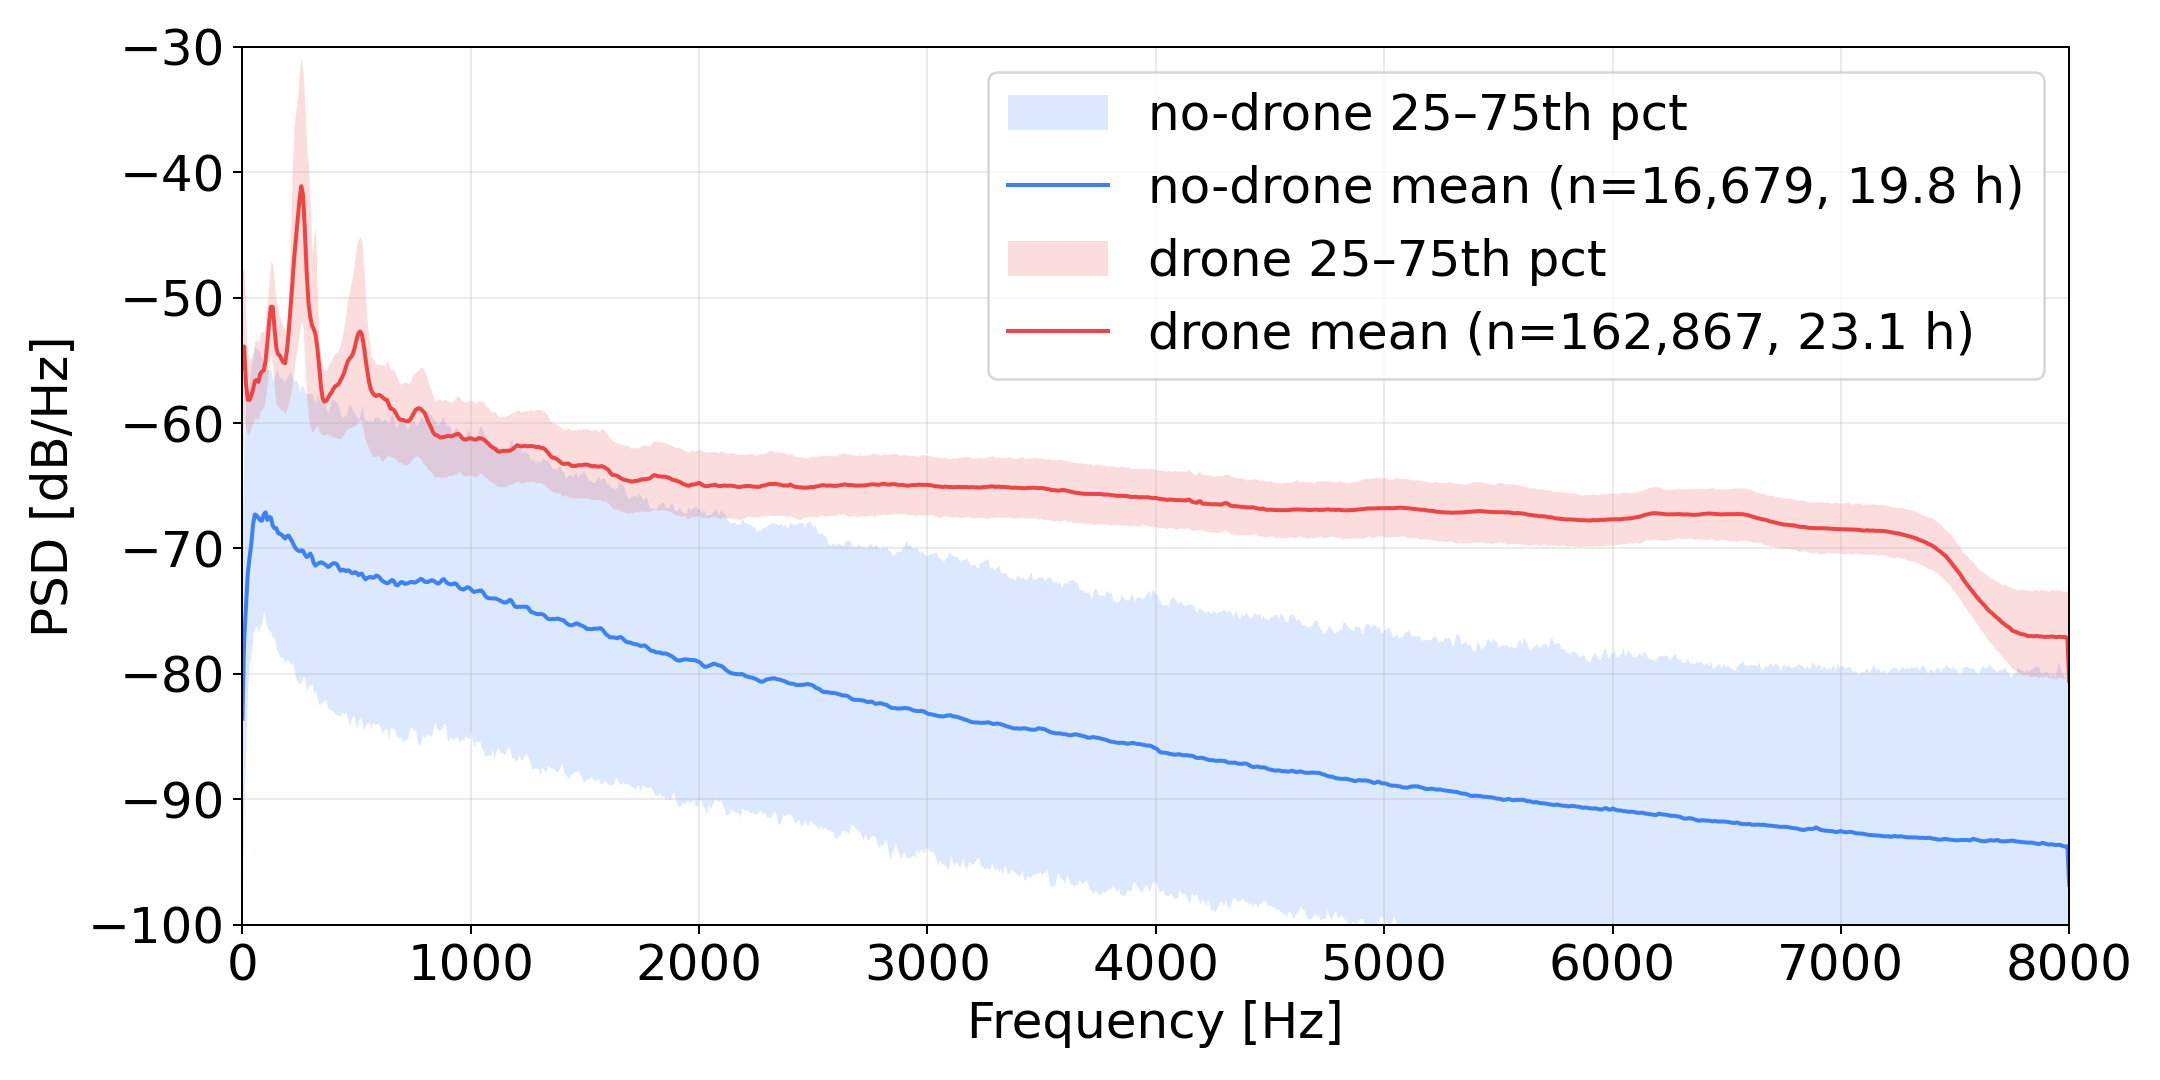
\includegraphics[width=\columnwidth]{figs/dads_average_spectrum.png}
  \caption{Mean PSD for drone ($n=163\,591$, red) and non-drone ($n=14\,868$, blue) recordings of the DADS dataset. The bands span the 25th to 75th percentile across recordings.}
  \label{fig:dads_spectrum}
\end{figure}

\subsection{Motor-derived references}
A motor signal is correlated with the order and tonal components of the noise, not with the broadband aerodynamic part: current, voltage, back-EMF, and Hall signals carry the electrical and mechanical state of the rotor, whereas the broadband noise also comes from turbulence and from the interaction with the airframe. Table~\ref{tab:real_references} lists the candidate sources.

\begin{table}[htbp]
\caption{Candidate motor-derived references}
\label{tab:real_references}
\centering
\scriptsize
\setlength{\tabcolsep}{3pt}
\begin{tabularx}{\columnwidth}{@{}>{\raggedright\arraybackslash}p{0.22\columnwidth}YY@{}}
\toprule
Source & Main properties and limits & Intended role \\
\midrule
Hall / encoder & Direct angle, deterministic pulses; needs a sensor and a common time base with the audio. & Preferred laboratory reference for the BPF and its order harmonics. \\
Rotor angle / back-EMF & Angle or commutation instants available in a sensorless ESC; unknown filtering and lower accuracy at low speed. & Practical source for synthesizing quadrature references. \\
DShot eRPM & Easy to integrate; conversion by pole count, quantization, and variable delay \cite{betaflightDshotRpm,ardupilotEscTelemetry}. & First prototype and diagnostics, not a standalone wideband reference. \\
Motor current & Carries commutation and load changes, but also PWM and switching noise. & Later comparison or complementary reference. \\
Reference microphone & Captures tonal and wideband noise; sensitive to airflow and acoustic feedback. & Comparison and hybrid wideband branch. \\
\bottomrule
\end{tabularx}
\end{table}

Rather than feeding a raw motor signal to the controller, the angle estimate $\theta[n]$ is turned into quadrature pairs for the BPF and selected harmonics,
\begin{equation}
 x_{k,c}[n]=\cos(k\theta[n]),\qquad
 x_{k,s}[n]=\sin(k\theta[n]),
 \label{eq:harmonic_reference}
\end{equation}
the standard basis of narrowband ANC for rotating machinery. A mismatch between the tachometric frequency and the actual tone lowers the attenuation \cite{xiao2006narrowband}, so the mechanical angle is converted to the BPF by the blade count and only harmonics with sufficient coherence against the microphone are kept. The telemetry also has to be time-aligned with the audio: the arrival time of each DShot frame is recorded, delay and jitter are measured, the eRPM to shaft-speed conversion is verified, and the audio ADC and the telemetry share a clock or the offset and drift are estimated continuously. Without that, the phase error grows with the harmonic order in~\eqref{eq:harmonic_reference}.

\section{FxLMS Controller}
\label{sec:method}
The feedforward model (Fig.~\ref{fig:fxlms_schema}) consists of a reference $x[n]$, a primary path $P(z)$ from the noise source to the microphone, an adaptive control filter $G(z)$ of length $L$, and a secondary path $C(z)$ from the actuator to the microphone. With the useful signal $s[n]$, the microphone signal and the error are
\begin{equation}
  d[n] = P(z)x[n] + s[n], \qquad e[n] = d[n] - C(z)y[n],
\end{equation}
where $y[n] = \sum_{i=0}^{L-1} g_i[n]x[n-i]$. A change of the weights reaches the microphone only through $C(z)$, so the adaptation uses the filtered reference $x'[n] = \hat{C}(z)x[n]$, with $\hat{C}(z)$ an estimate of the secondary path, and the normalized update
\begin{equation}
  g_i[n+1] = g_i[n] + \frac{\mu}{P[n]}\, e[n]\,x'[n-i],
  \label{eq:fxlms_update}
\end{equation}
\begin{equation}
  P[n] = \varepsilon + \sum_{i=0}^{L-1} {x'}^2[n-i].
  \label{eq:fxlms_power}
\end{equation}
The normalization by the reference power $P[n]$ removes the dependence of the step on the input level, so the dimensionless $\mu$ (about 0.09 here) does not have to be retuned per operating point; $\varepsilon$ guards against a weak reference.

\begin{figure}[htbp]
  \centering
  \includegraphics[width=\columnwidth]{figs/fxlms_schema.pdf}
  \caption{Block diagram of the FxLMS algorithm with the secondary path model $\hat{C}(z)$.}
  \label{fig:fxlms_schema}
\end{figure}

With $R$ motor references and $A$ actuators the controller holds $A\times R$ adaptive filters; the output of actuator $a$ sums the contributions of all references, all filters learn from the same error, and each uses its own filtered reference $x'_{a,r}[n]=\hat{C}_a(z)x_r[n]$. The normalization power is then summed over all reference-actuator pairs,
\begin{equation}
  P[n] = \varepsilon + \sum_{a=0}^{A-1}\sum_{r=0}^{R-1}\sum_{i=0}^{L-1} {x'}_{a,r}^2[n-i],
  \label{eq:fxlms_power_multi}
\end{equation}
so the effective step shrinks with the channel count while $\mu$ stays the same. The alternative of adding the motor references before the controller (a single reference channel) discards the per-motor phase information, which the multi-reference form keeps.

The controller is written in C for the flight-control microcontroller. Samples and coefficients are \texttt{int16\_t} in Q15; the FIR accumulates in a wider type and shifts by 15 bits, the weight update runs in 64-bit arithmetic and saturates the increment. The power $P[n]$ is a running sum of squares over the window, updated in $O(1)$ per channel by subtracting the oldest square and adding the newest. The core allocates nothing; the caller supplies a state buffer sized for the configuration.

\section{Evaluation Methodology}
\label{sec:setup}
The controller is judged on the error signal over a window placed after the adaptation transient: the impulsive event has to survive it while the component correlated with the motors drops. The ego-noise attenuation is
\begin{equation}
  A_{\mathrm{drone}} = 10\log_{10}\frac{\mathrm{MSE}(d_{\mathrm{drone}})}{\mathrm{MSE}(e-s)},
  \label{eq:drone_atten}
\end{equation}
with $d_{\mathrm{drone}}$ the ego-noise component at the microphone and $e-s$ the residual noise. Per frequency, $A(f)=\mathrm{PSD}_{d_{\mathrm{drone}}}(f)-\mathrm{PSD}_{e-s}(f)$ from Welch estimates (4096-sample Hann window, 50\,\% overlap) is reported over the whole band, so that frequencies where the controller adds energy are visible next to those where it removes it; its energy-weighted average equals~\eqref{eq:drone_atten}. Detection performance is measured separately, by comparing correct and false detections of a short-term-energy detector before and after the controller.

Validation starts with a static single-rotor test: during a controlled speed sweep the sound, the time-stamped speed or angle, the motor current, and the ESC control signal are recorded together, the coherence of every candidate reference with the BPF harmonics is measured, and at the same operating points the attenuation per order, the convergence, and any amplification outside the target tones are compared. A multi-rotor and a tethered-hover test follow, adding differing speeds, mutual acoustic paths, and load changes.
% TODO: fill in the actual rig (motor, ESC, propeller, microphone, secondary
% source, sampling), the secondary-path identification, and the event source
% once the campaign is done.

\section{Results}
\label{sec:results}
% TODO: measured results from the campaign: attenuation per harmonic order and
% in total, convergence, effect on impulsive-event detection.

\section{Conclusion}
\label{sec:conclusion}
% TODO: write from the measured results.

\bibliographystyle{IEEEtran}
\bibliography{references}

\end{document}
